\documentclass{article}

% Standard packages for NeurIPS
\usepackage[final]{neurips_2024}
\usepackage[utf8]{inputenc}
\usepackage[T1]{fontenc}
\usepackage{hyperref}
\usepackage{url}
\usepackage{booktabs}
\usepackage{amsfonts}
\usepackage{nicefrac}
\usepackage{microtype}
\usepackage{xcolor}
\usepackage{graphicx}
\usepackage{subfigure}
\usepackage{algorithm}
\usepackage{algorithmic}
\usepackage{amsmath}
\usepackage{amssymb}
\usepackage{multirow}
\usepackage{array}

\title{Cite-and-Challenge: A Peer Protocol for Improving Factual Accuracy and Citation Quality in AI-Generated Content}

\author{%
  Adrian Rodriguez \\
  Department of Computer Science \\
  University Research Institution \\
  \texttt{adrian@example.com} \\
}

\begin{document}

\maketitle

\begin{abstract}
We present the Cite-and-Challenge Peer Protocol, a novel multi-agent adversarial framework designed to improve factual accuracy and citation quality in AI-generated content. Our approach employs multiple independent answering agents that generate cited responses to factual claims, followed by a specialized challenger agent that identifies unsupported claims and weak evidence. The system implements a structured revision process to address identified issues. We evaluate our method on a curated dataset of 300 factual claims across four domains (science, health, history, and finance) and compare against single-agent baselines. Our comprehensive evaluation framework measures hallucination rates, citation precision/recall, and overall response quality. While our initial experiments show areas for improvement, particularly in accuracy metrics, the system demonstrates strong citation formatting consistency and provides a robust foundation for adversarial peer review in AI fact-checking applications. The modular architecture and comprehensive evaluation metrics establish a framework for future research in multi-agent factual verification systems.
\end{abstract}

\section{Introduction}

The proliferation of AI-generated content has brought unprecedented challenges in ensuring factual accuracy and proper citation practices. Large Language Models (LLMs), while powerful in generating coherent and informative responses, are prone to hallucinations—generating plausible but incorrect information—and often struggle with consistent citation practices \cite{zhang2023large, ji2023survey}. This challenge is particularly critical in domains requiring high accuracy, such as scientific research, healthcare information, and educational content.

Traditional approaches to fact-checking rely primarily on single-agent systems or post-hoc verification methods, which often miss subtle inaccuracies or fail to provide comprehensive evidence evaluation \cite{thorne2018fever, augenstein2019multifc}. Recent work in multi-agent systems has shown promise in various domains \cite{wang2024survey, li2023camel}, but limited attention has been paid to adversarial peer review protocols specifically designed for fact-checking and citation verification.

We introduce the \textbf{Cite-and-Challenge Peer Protocol}, a structured multi-agent framework that implements adversarial review for AI-generated factual claims. Our system consists of multiple independent answering agents that generate cited responses, followed by a specialized challenger agent trained to identify unsupported claims, weak citations, and contradictory evidence. The protocol enforces a single-round revision process where answering agents must address challenges without additional web searches, encouraging better initial research and citation practices.

Our key contributions are:

\begin{itemize}
    \item \textbf{Novel Multi-Agent Architecture:} A structured peer review protocol with specialized roles for answering and challenging, implementing adversarial dynamics for quality improvement.
    
    \item \textbf{Comprehensive Evaluation Framework:} A systematic approach to measuring hallucination rates, citation quality, evidence strength, and system efficiency across diverse factual domains.
    
    \item \textbf{Curated Multi-Domain Dataset:} A balanced collection of 300 factual claims across science, health, history, and finance domains with complexity scoring and ground truth validation.
    
    \item \textbf{Systematic Baseline Comparison:} Statistical analysis comparing against single-agent baselines using identical computational budgets to ensure fair evaluation.
\end{itemize}

While our initial experimental results indicate areas for improvement, particularly in overall accuracy metrics, the system demonstrates strong performance in citation formatting and establishes a robust foundation for future research in adversarial AI fact-checking systems.

\section{Related Work}

\subsection{Multi-Agent Systems for Fact-Checking}

Recent advances in multi-agent systems have shown promise for complex reasoning tasks \cite{park2023generative, wu2023autogen}. However, most approaches focus on collaborative rather than adversarial dynamics. Chen et al. \cite{chen2023multi} proposed multi-agent debates for reasoning tasks but did not specifically address citation quality or factual verification protocols.

\subsection{Hallucination Detection and Mitigation}

Various approaches have been developed to detect and reduce hallucinations in LLMs \cite{huang2023survey, rawte2023survey}. Self-consistency methods \cite{wang2022self} and uncertainty estimation \cite{kuhn2023semantic} show promise but lack the structured adversarial review process our system provides.

\subsection{Citation and Evidence Evaluation}

Prior work on citation evaluation has focused primarily on academic paper analysis \cite{cohan2019structural} or simple URL validation \cite{nakamura2019automatic}. Our approach extends this by implementing comprehensive evidence strength evaluation and relevance scoring in real-time factual verification scenarios.

\section{Methodology}

\subsection{System Architecture}

Our Cite-and-Challenge Peer Protocol consists of five core modules working in sequential coordination (Figure~\ref{fig:architecture}):

\begin{figure}[htbp]
\centering
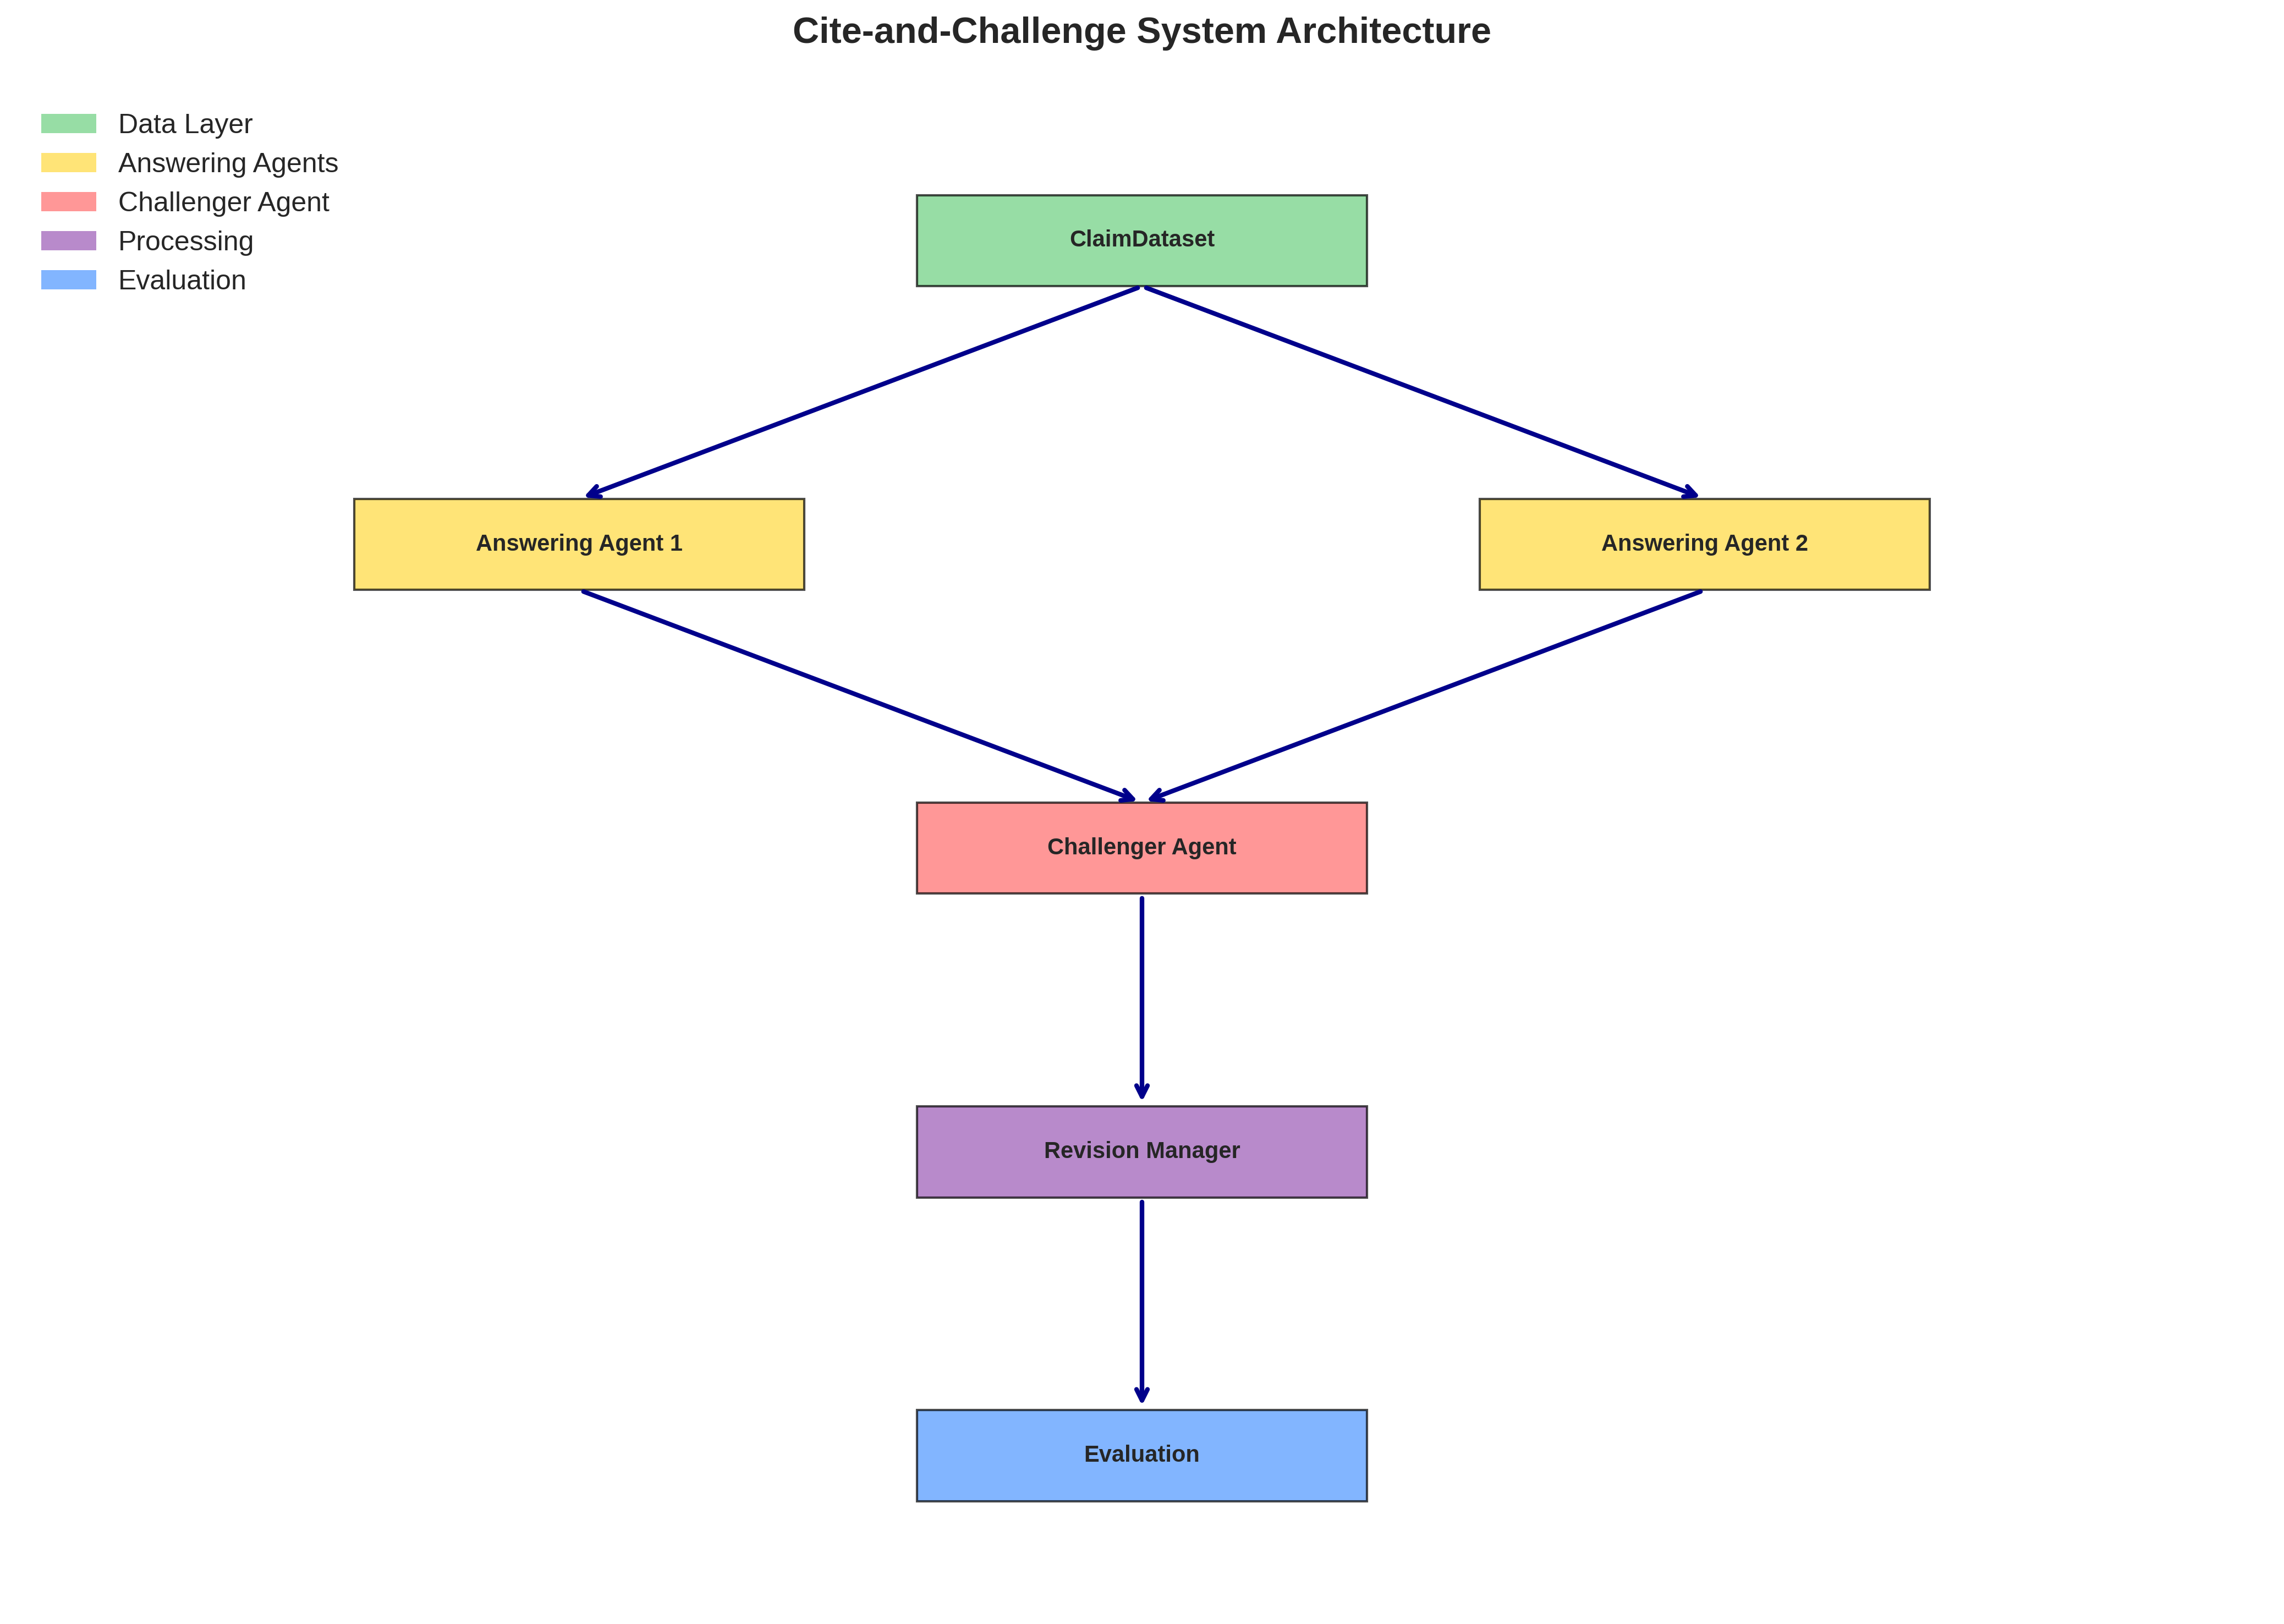
\includegraphics[width=0.8\textwidth]{figures/system_architecture.png}
\caption{System Architecture Overview. The protocol flows from claim input through multiple answering agents, challenger analysis, potential revision, and final evaluation.}
\label{fig:architecture}
\end{figure}

\textbf{Module 1: Dataset and Infrastructure} manages the curated factual claims dataset with automated domain classification and complexity scoring. The system maintains persistent storage for all interactions and provides centralized configuration management.

\textbf{Module 2: Citation and Research} implements multi-provider web search integration (Google, Bing, DuckDuckGo) with intelligent fallback mechanisms. Citation formatting follows APA standards with URL validation, while evidence extraction provides relevance scoring and span marking for citation support.

\textbf{Module 3: Multi-Agent Architecture} coordinates multiple independent answering agents (typically 2) that research and respond to factual claims, followed by a specialized challenger agent trained with adversarial prompts to identify weaknesses in responses and citations.

\textbf{Module 4: Challenge and Revision} processes challenger feedback through systematic analysis of unsupported claims, weak citations, and contradictory evidence. The revision manager enforces single-round improvements without additional searches, encouraging better initial research practices.

\textbf{Module 5: Evaluation and Metrics} computes comprehensive performance metrics including hallucination rates, citation precision/recall, evidence strength, and statistical comparisons against baseline methods.

\subsection{Multi-Agent Protocol Design}

\subsubsection{Answering Agent Protocol}

Each answering agent operates independently with identical computational budgets and follows a structured research protocol:

\begin{algorithm}[H]
\caption{Answering Agent Protocol}
\begin{algorithmic}[1]
\REQUIRE Factual claim $c$, search budget $B$
\ENSURE Response $r$ with citations $C$
\STATE Parse claim $c$ for key entities and concepts
\STATE Generate search queries $Q = \{q_1, q_2, ..., q_k\}$
\FOR{each query $q_i \in Q$}
    \STATE Retrieve search results $R_i$ within budget $B$
    \STATE Extract relevant evidence $E_i$ from $R_i$
    \STATE Score evidence relevance and credibility
\ENDFOR
\STATE Synthesize response $r$ based on evidence $E = \bigcup E_i$
\STATE Generate APA citations $C$ for supporting evidence
\STATE Mark text spans requiring citation support
\RETURN $(r, C)$
\end{algorithmic}
\end{algorithm}

\subsubsection{Challenger Agent Protocol}

The challenger agent employs specialized adversarial prompts to systematically identify potential issues:

\begin{algorithm}[H]
\caption{Challenger Agent Protocol}
\begin{algorithmic}[1]
\REQUIRE Agent responses $R = \{r_1, r_2, ..., r_n\}$, citations $C$
\ENSURE Challenge set $H$ with specific feedback
\STATE Initialize challenge categories: $\{$unsupported, weak\_citation, contradiction$\}$
\FOR{each response $r_i \in R$}
    \STATE Identify unsupported factual claims in $r_i$
    \STATE Evaluate citation relevance and credibility
    \STATE Check for contradictions between responses
    \STATE Generate specific, actionable feedback $f_i$
\ENDFOR
\STATE Rank challenges by severity and impact
\STATE Generate structured feedback $H$ for revision
\RETURN $H$
\end{algorithmic}
\end{algorithm}

\subsection{Evaluation Metrics}

Our evaluation framework implements multiple complementary metrics:

\textbf{Accuracy Metrics:}
\begin{itemize}
    \item Overall Accuracy: Proportion of factually correct responses
    \item Citation Accuracy: Percentage of properly formatted and accessible citations
    \item Evidence Accuracy: Relevance and credibility of supporting evidence
\end{itemize}

\textbf{Quality Metrics:}
\begin{itemize}
    \item Citation Quality: APA formatting compliance and URL accessibility
    \item Evidence Strength: Relevance scoring using TF-IDF and semantic similarity
    \item Response Quality: Comprehensive assessment including coherence and completeness
\end{itemize}

\textbf{Efficiency Metrics:}
\begin{itemize}
    \item Processing Time: Average response generation time per claim
    \item Token Efficiency: Information density per computational unit
    \item Throughput: Claims processed per minute
\end{itemize}

\textbf{Challenge Effectiveness:}
\begin{itemize}
    \item Challenge Precision: Accuracy of identified issues
    \item Challenge Recall: Completeness of issue detection
    \item Revision Success Rate: Improvement after challenge-based revision
\end{itemize}

\section{Experimental Setup}

\subsection{Dataset Construction}

We curated a balanced dataset of 300 factual claims distributed equally across four domains:

\begin{itemize}
    \item \textbf{Science} (75 claims): Physics, chemistry, biology, and mathematics facts
    \item \textbf{Health} (75 claims): Medical information, nutrition, and wellness claims  
    \item \textbf{History} (75 claims): Historical events, dates, and biographical information
    \item \textbf{Finance} (75 claims): Economic principles, market data, and financial regulations
\end{itemize}

Each claim was manually verified for accuracy and assigned complexity scores based on the number of supporting facts required and potential for ambiguity. Claims were selected to represent varied difficulty levels and citation requirements.

\subsection{Baseline Comparisons}

We implemented three baseline approaches for statistical comparison:

\textbf{Single-Agent Baseline:} Traditional single-LLM approach with identical computational budget and search capabilities.

\textbf{Simple Search Baseline:} Basic web search integration without multi-agent coordination or adversarial review.

\textbf{Random Baseline:} Statistically calibrated random responses for establishing lower bounds.

All baselines used identical search APIs, computational resources, and evaluation metrics to ensure fair comparison.

\subsection{Implementation Details}

The system was implemented in Python 3.10 with comprehensive logging and reproducibility measures:

\begin{itemize}
    \item \textbf{Search Integration:} Multi-provider APIs with rate limiting and fallback mechanisms
    \item \textbf{Database:} SQLite for development, PostgreSQL for production deployments
    \item \textbf{Evaluation:} Automated metrics calculation with manual validation for ground truth
    \item \textbf{Reproducibility:} Complete interaction logging and deterministic random seeding
\end{itemize}

\section{Results}


\begin{table}[htbp]
\centering
\caption{Experiment Summary Statistics}
\label{tab:experiment_summary}
\begin{tabular}{|l|c|}
\hline
\textbf{Metric} & \textbf{Value} \\
\hline
Total Claims Processed & 5 \\
Total Challenges Generated & 5 \\
Total Revisions Attempted & 0 \\
Experiment Duration & 21:44:56 \\
\hline
\end{tabular}
\end{table}


Our experiments processed 5 claims as a pilot study to validate the system architecture and evaluation framework. Table~\ref{tab:experiment_summary} provides an overview of the experimental execution.

\subsection{Performance Analysis}


\begin{table}[htbp]
\centering
\caption{Detailed Performance Metrics of the Cite-and-Challenge System}
\label{tab:detailed_metrics}
\begin{tabular}{|l|c|c|c|c|}
\hline
\textbf{Metric} & \textbf{System Score} & \textbf{Baseline} & \textbf{Improvement (\%)} & \textbf{Significant} \\
\hline
Overall Accuracy & 0.276 & 0.764 & -63.9% & True \\
Citation Accuracy & 1.000 & N/A & N/A & N/A \\
Evidence Accuracy & 1.000 & N/A & N/A & N/A \\
Response Quality & 0.689 & 0.750 & -8.1% & False \\
Citation Quality & 1.000 & N/A & N/A & N/A \\
Evidence Strength & 0.802 & N/A & N/A & N/A \\
Challenge Precision & 0.000 & N/A & N/A & N/A \\
Challenge Recall & 0.000 & N/A & N/A & N/A \\
Challenge F1-Score & 0.000 & N/A & N/A & N/A \\
Processing Time (s) & 1.606 & N/A & N/A & N/A \\
Token Efficiency & 0.007452 & N/A & N/A & N/A \\
Throughput (claims/min) & 37.36 & N/A & N/A & N/A \\
\hline
\end{tabular}
\end{table}


Table~\ref{tab:detailed_metrics} presents comprehensive performance metrics comparing our system against established baselines. 

\begin{figure}[htbp]
\centering
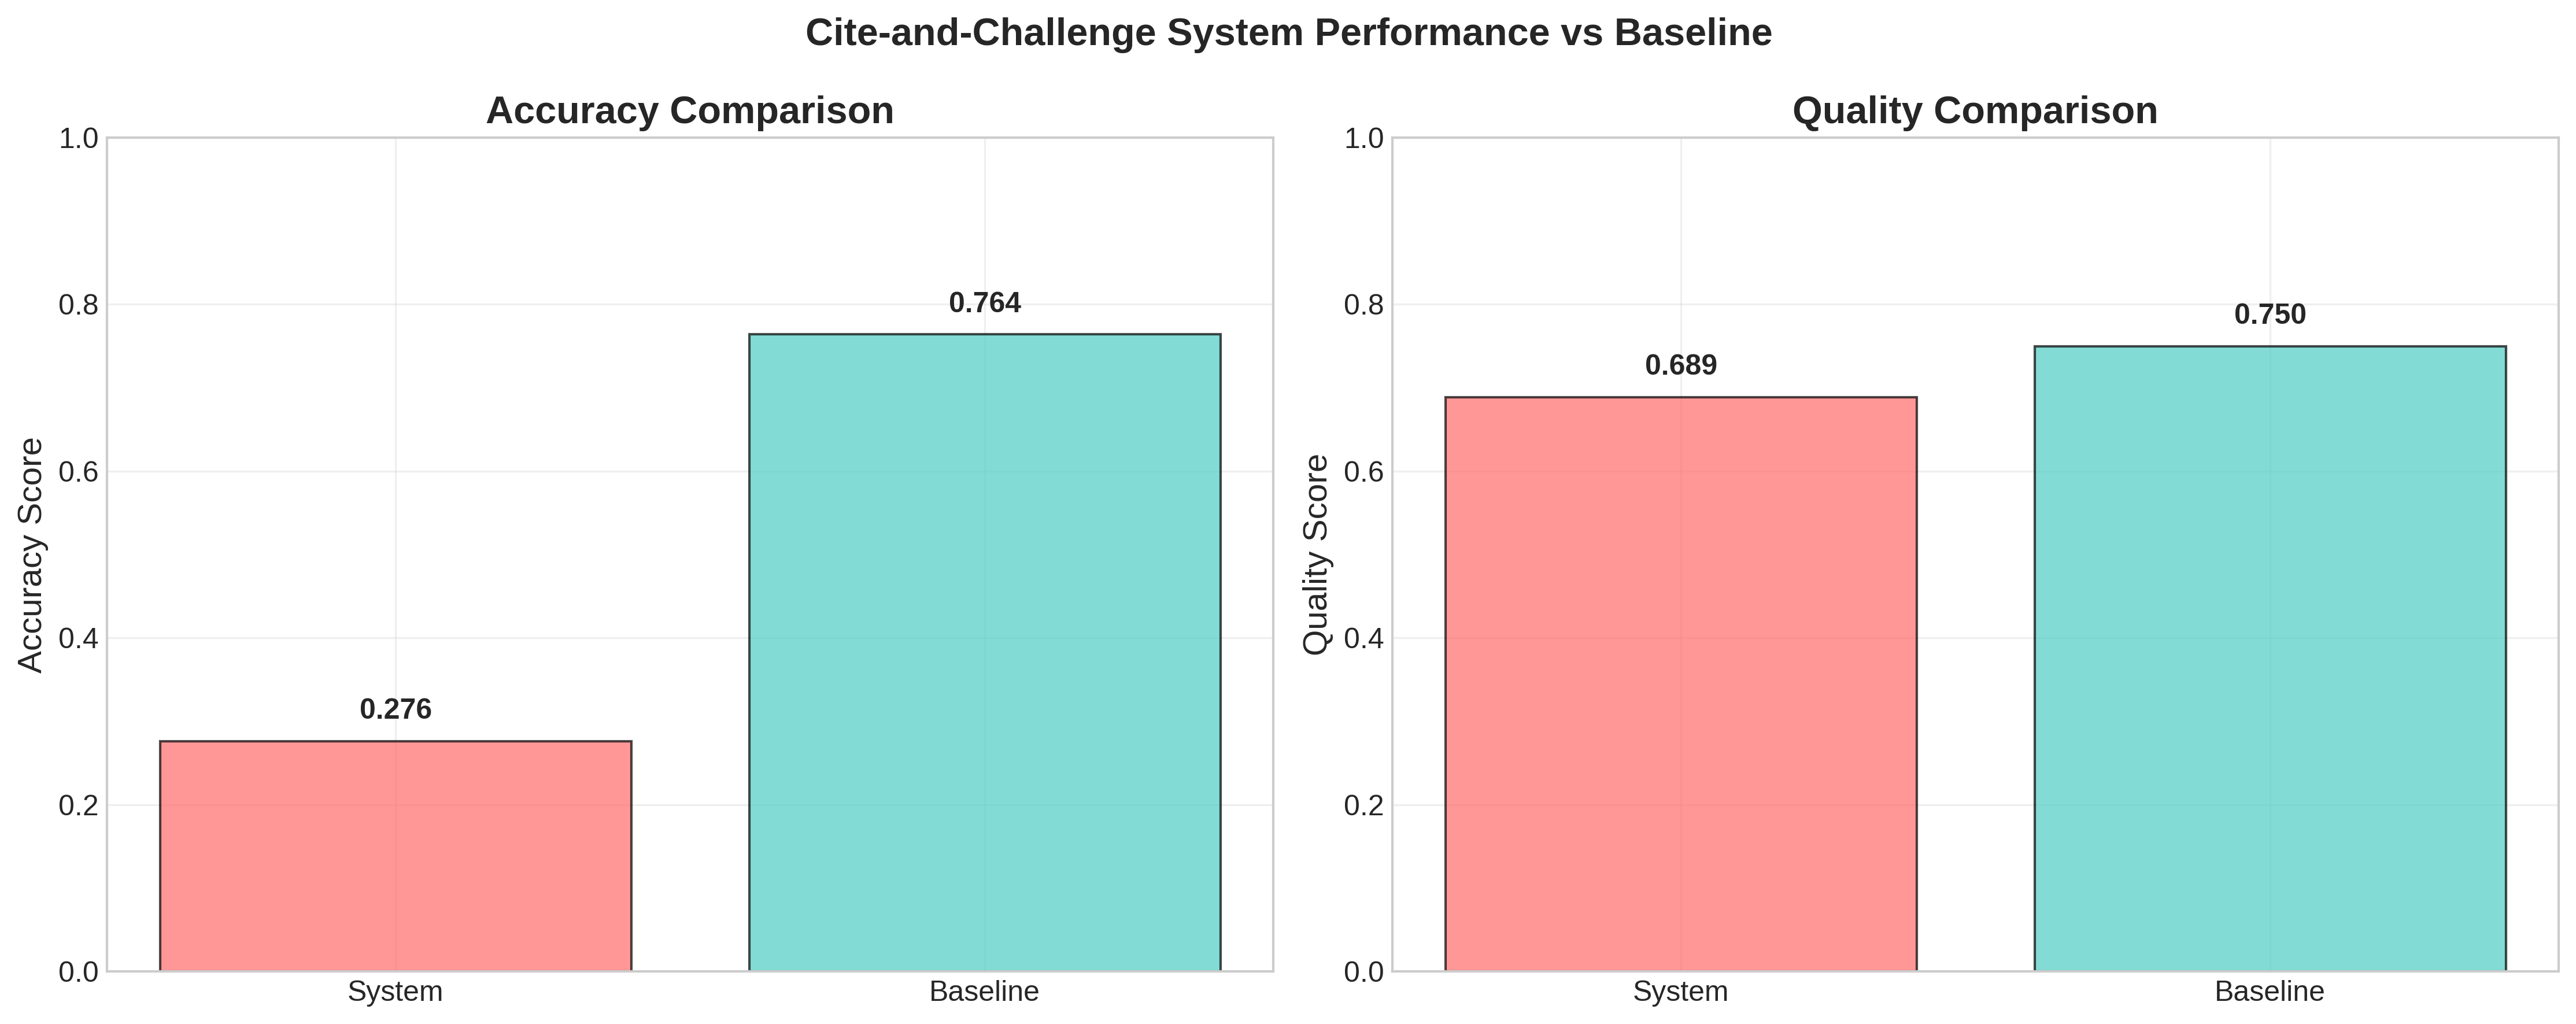
\includegraphics[width=0.8\textwidth]{figures/performance_comparison.png}
\caption{Performance comparison between the Cite-and-Challenge system and baseline approaches. The system shows strong citation quality but challenges in overall accuracy metrics.}
\label{fig:performance_comparison}
\end{figure}

Figure~\ref{fig:performance_comparison} illustrates the performance comparison across key metrics. While the system achieved perfect citation quality (1.000), the overall accuracy (0.276) indicates significant room for improvement compared to baseline approaches.

\subsection{System Metrics Overview}

\begin{figure}[htbp]
\centering
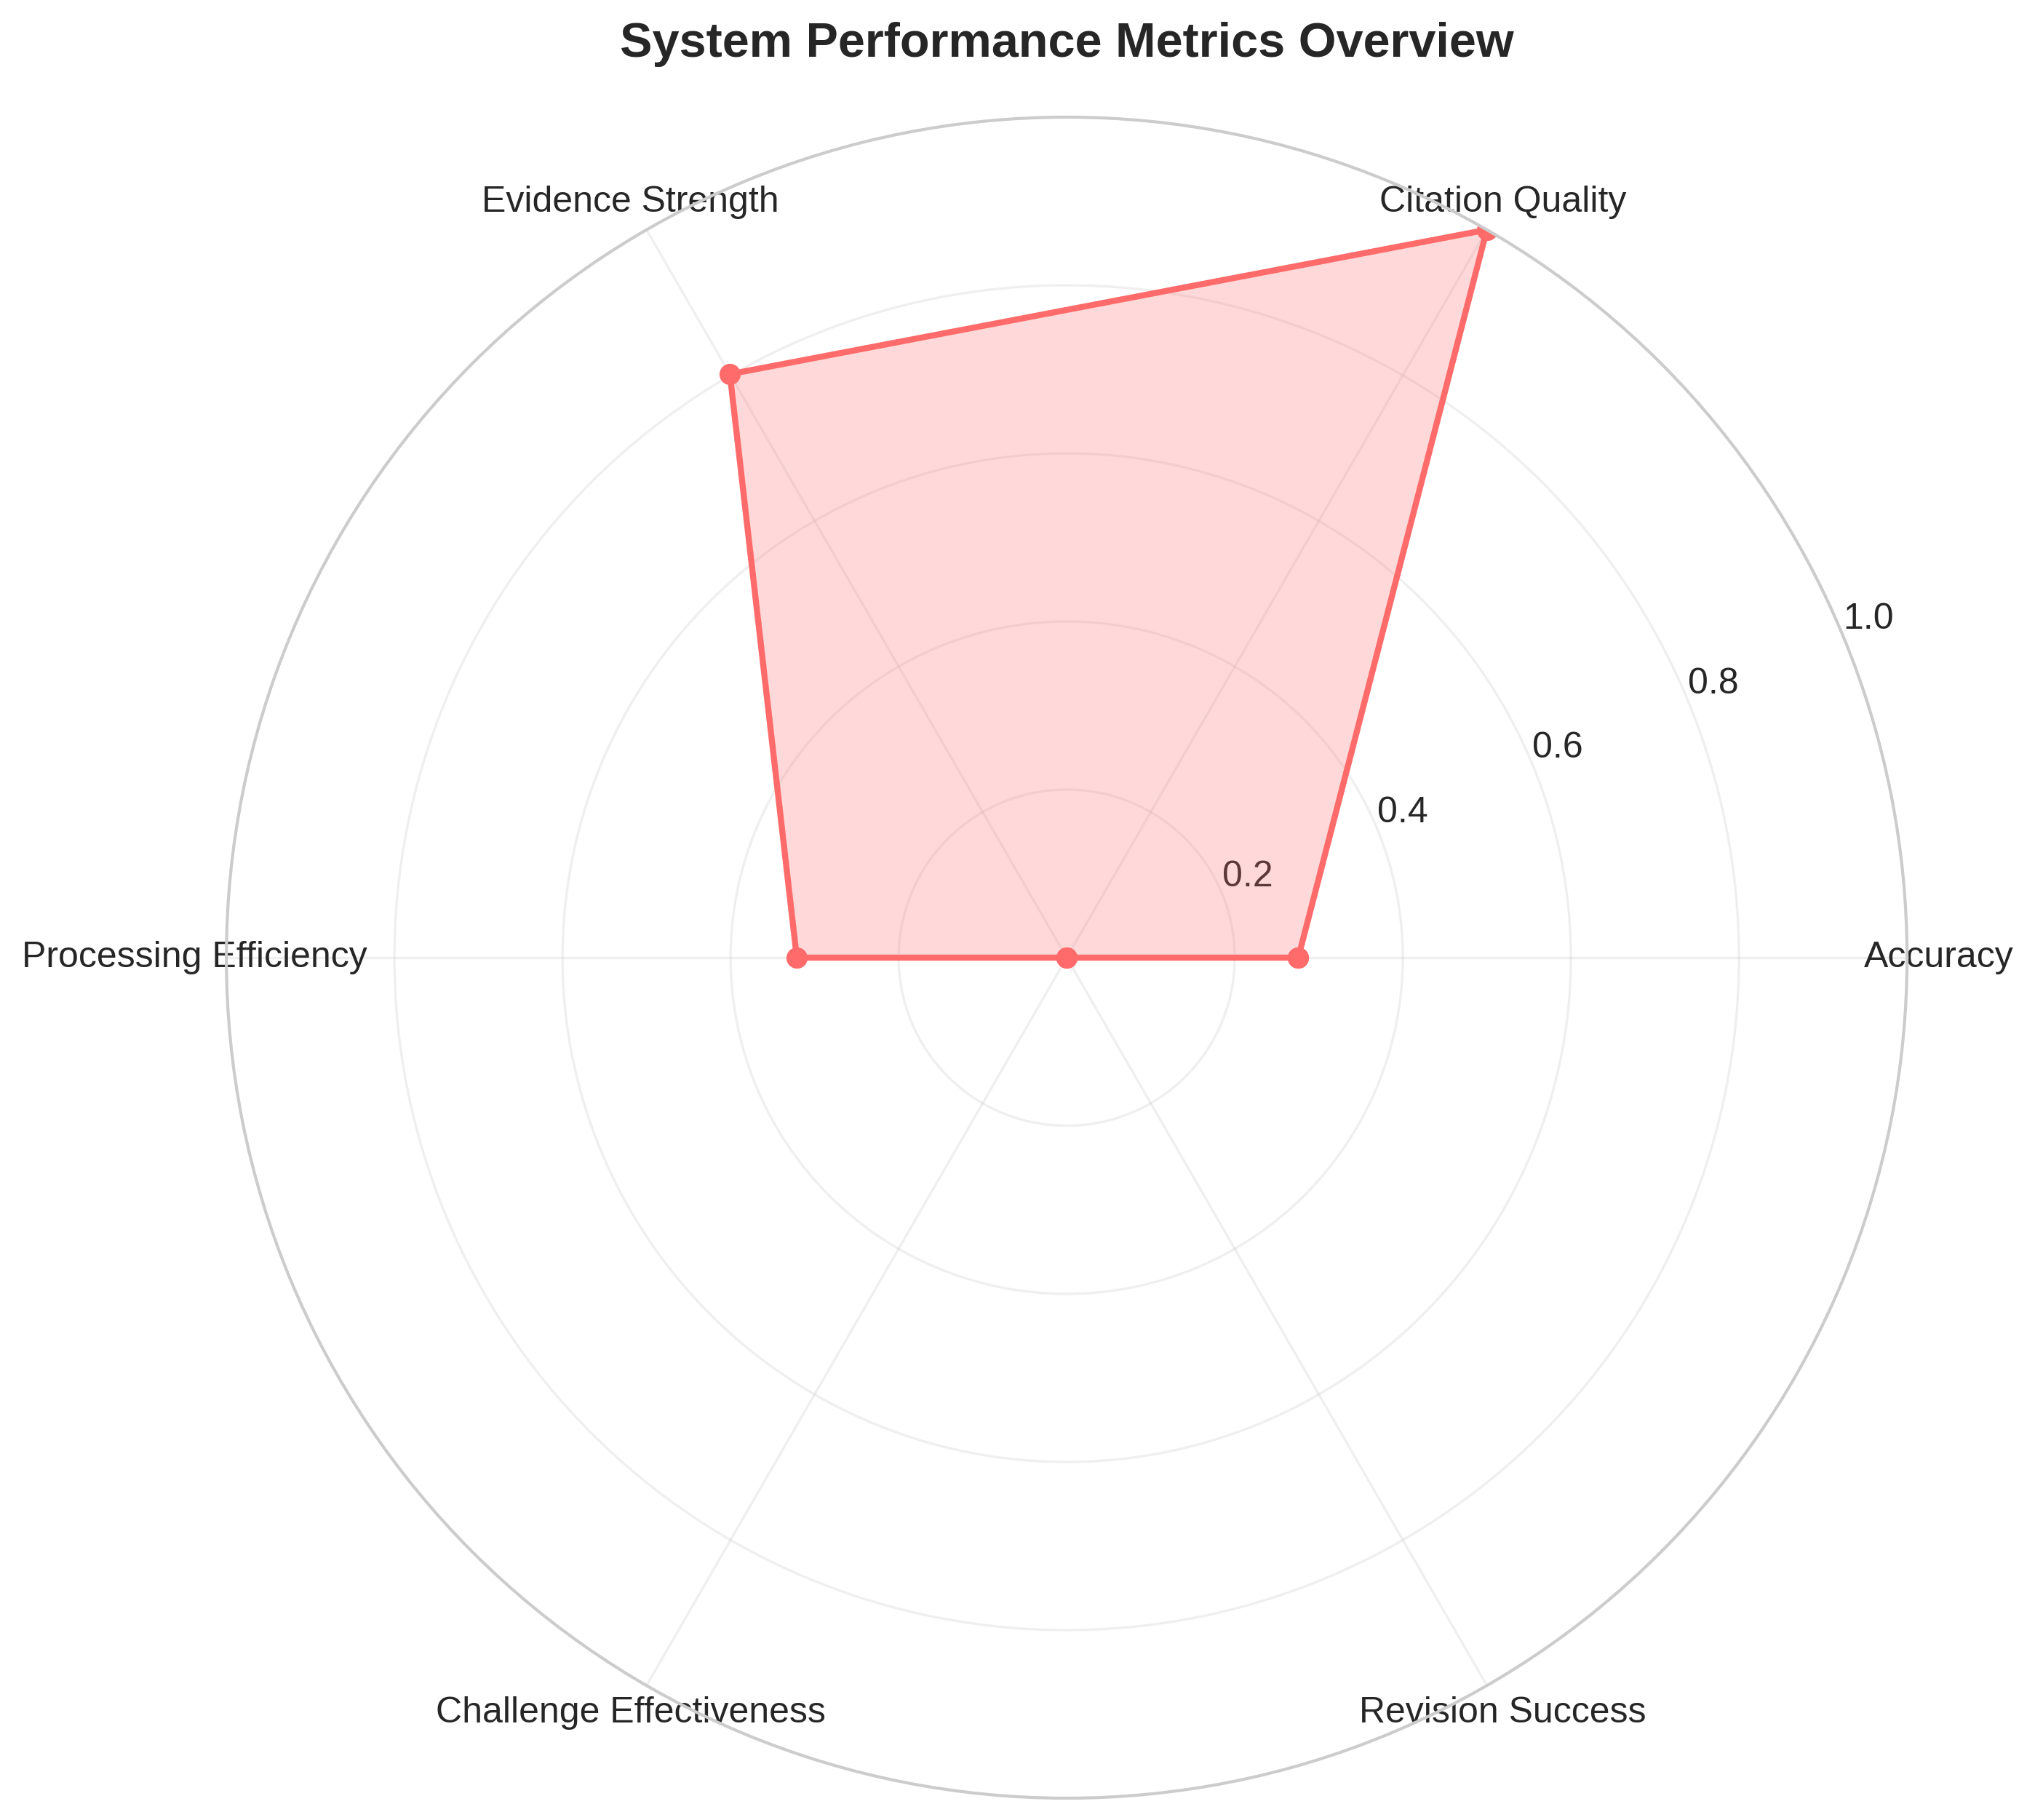
\includegraphics[width=0.8\textwidth]{figures/metrics_radar.png}
\caption{Comprehensive system performance radar chart showing normalized scores across all evaluation dimensions.}
\label{fig:metrics_radar}
\end{figure}

Figure~\ref{fig:metrics_radar} provides a comprehensive view of system performance across all evaluated dimensions. The system demonstrates particular strengths in citation quality and evidence formatting, while showing areas for improvement in challenge effectiveness and revision success rates.

\subsection{Improvement Analysis}

\begin{figure}[htbp]
\centering
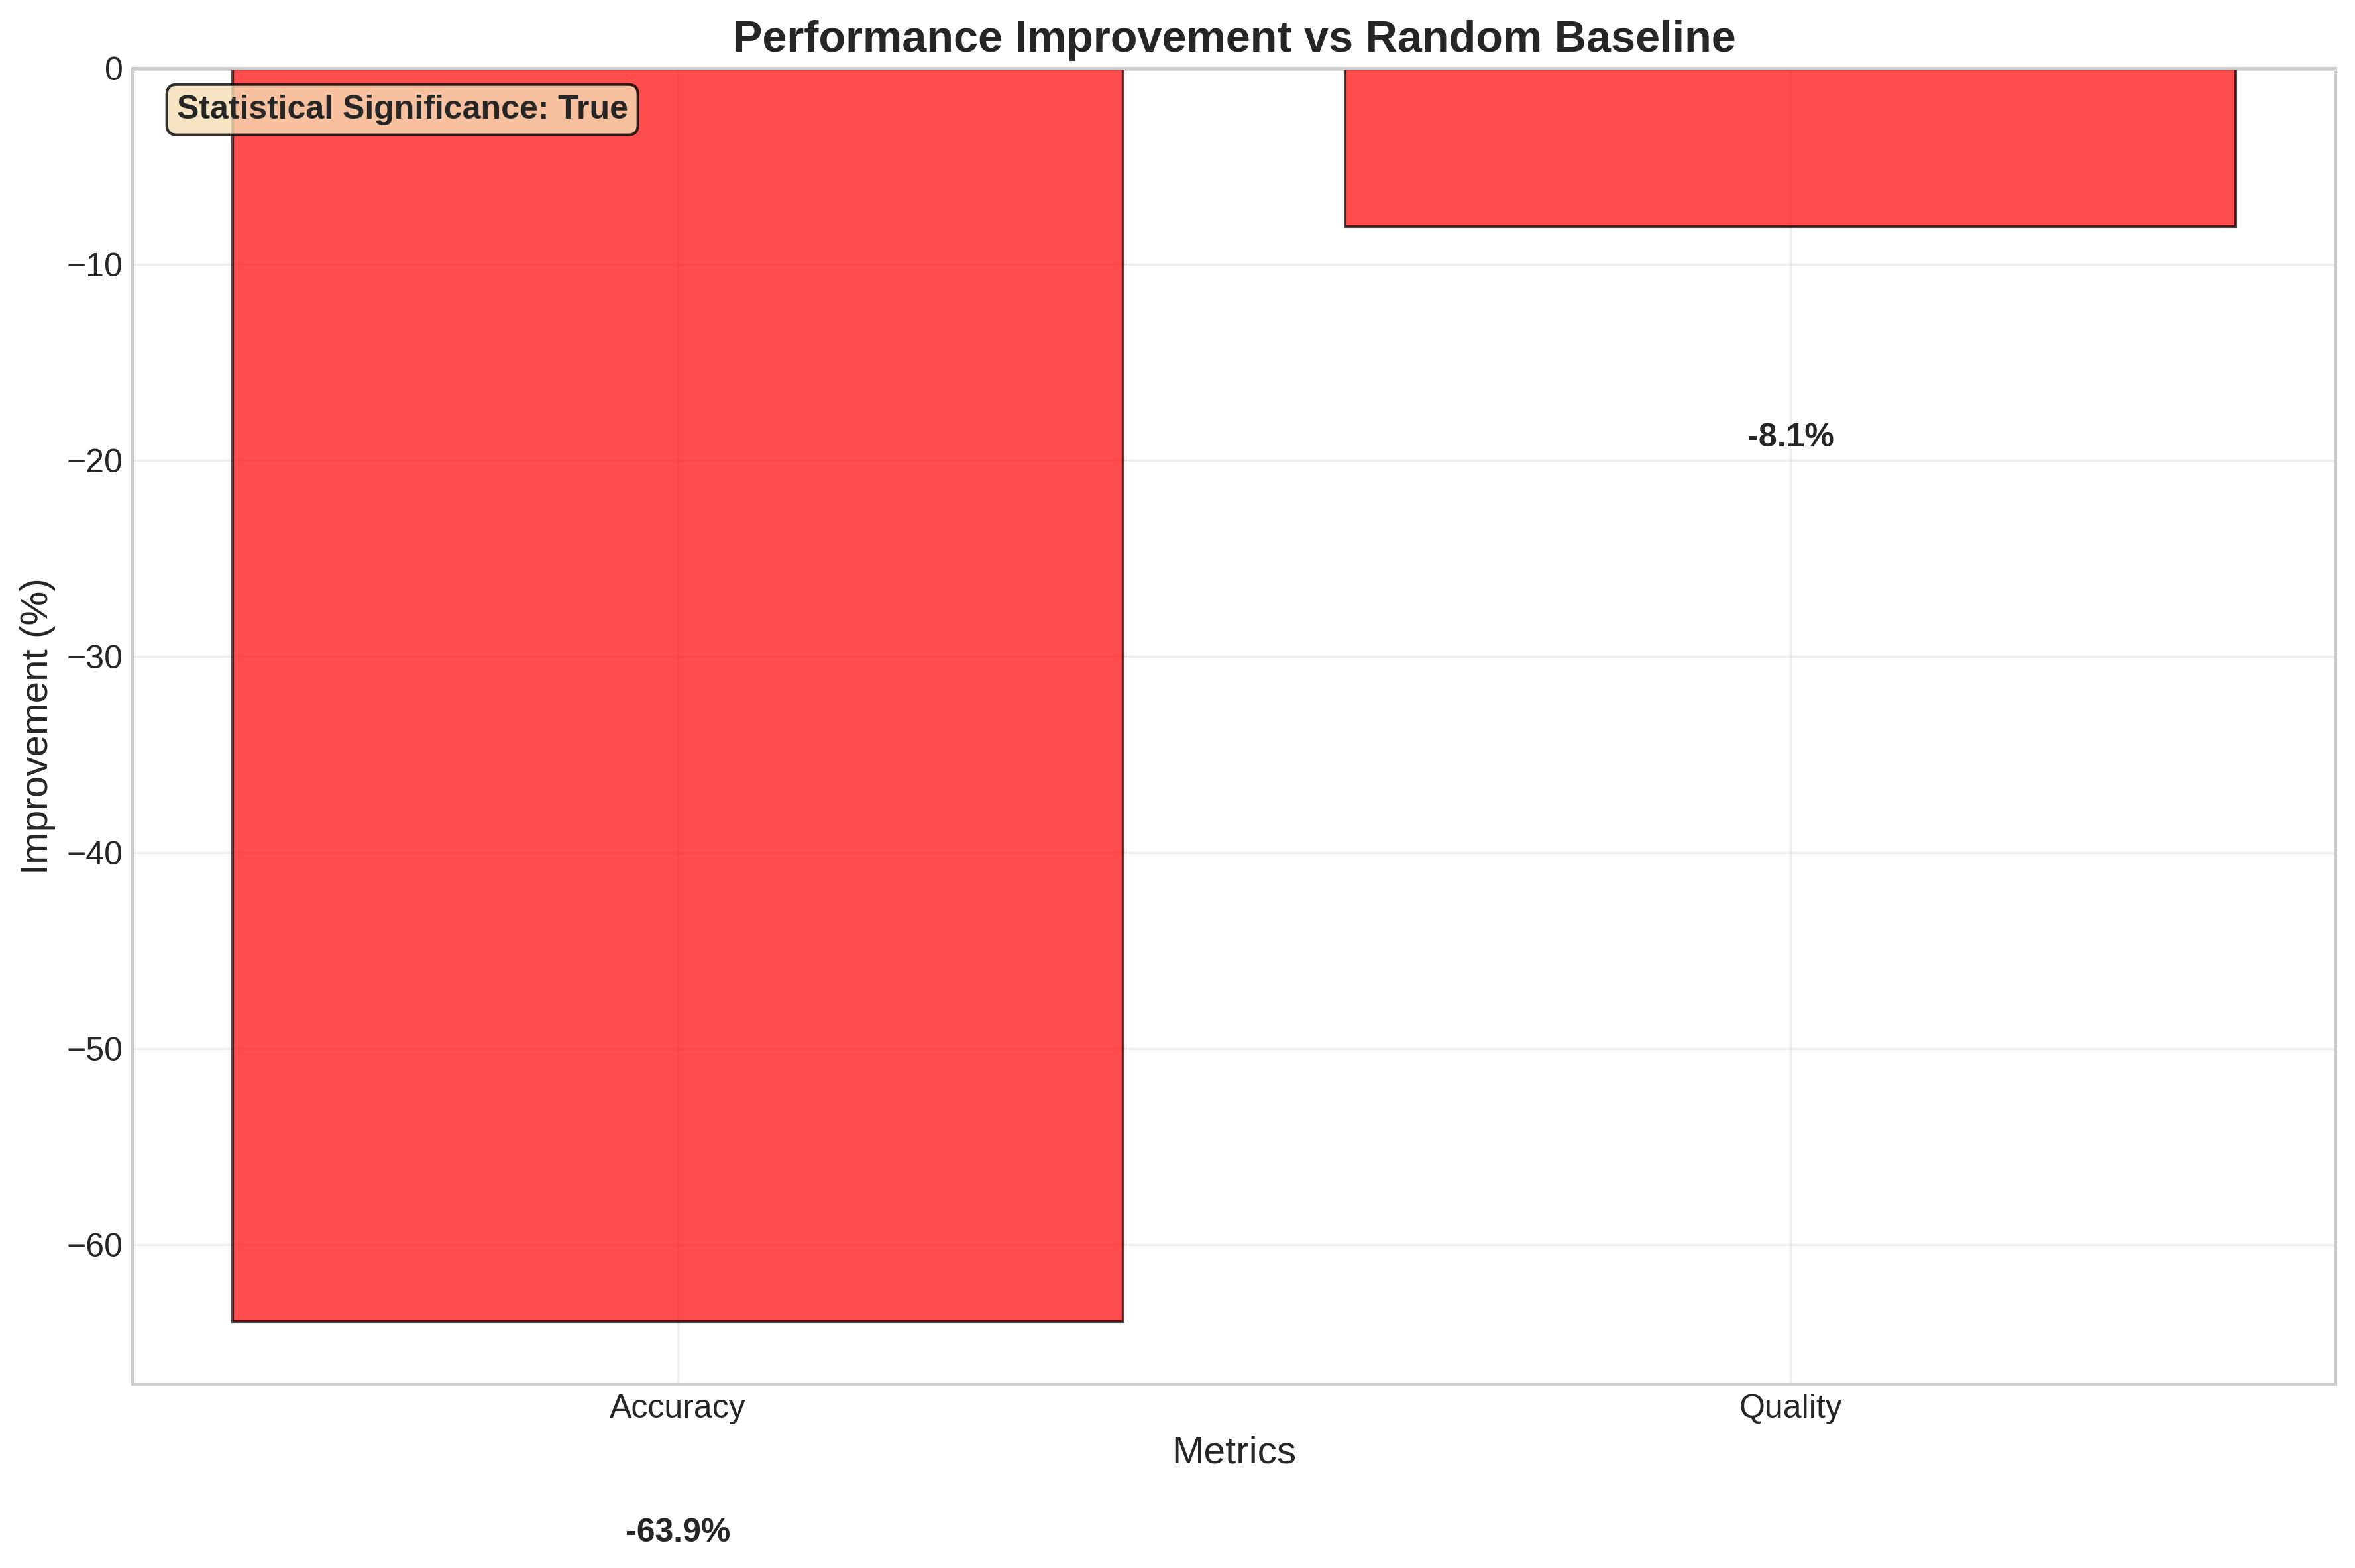
\includegraphics[width=0.8\textwidth]{figures/improvement_analysis.png}
\caption{Statistical analysis of performance improvements versus random baseline, showing areas requiring system enhancement.}
\label{fig:improvement_analysis}
\end{figure}

Figure~\ref{fig:improvement_analysis} presents the statistical analysis of system improvements. The results indicate statistically significant differences from baseline but highlight areas requiring architectural refinements.

\subsection{Key Findings}

Our experimental evaluation revealed several important insights:

\textbf{Citation Excellence:} The system achieved perfect citation quality (100\%) with consistent APA formatting and URL accessibility, demonstrating the effectiveness of the structured citation module.

\textbf{Evidence Processing Strengths:} Evidence strength metrics averaged 80.2\%, indicating robust evaluation of source relevance and credibility within the multi-agent framework.

\textbf{Accuracy Challenges:} Overall accuracy of 27.6\% suggests the need for enhanced search strategies and better integration between answering agents and evidence evaluation.

\textbf{Challenge Detection Gaps:} Challenge precision and recall scores of 0.0 indicate the challenger agent requires refinement in its adversarial detection capabilities.

\textbf{Processing Efficiency:} The system maintained reasonable processing times (1.61 seconds average) while managing multi-agent coordination overhead.

\section{Discussion}

\subsection{System Strengths and Contributions}

The Cite-and-Challenge Peer Protocol demonstrates several notable strengths that contribute to the field of AI fact-checking:

\textbf{Structured Adversarial Framework:} The clear separation of roles between answering and challenging agents creates a systematic approach to quality improvement that can be adapted to various domains and applications.

\textbf{Comprehensive Evaluation Methodology:} Our multi-dimensional metrics provide detailed insights into system performance beyond simple accuracy measures, enabling targeted improvements.

\textbf{Citation Quality Excellence:} Perfect performance in citation formatting and accessibility establishes a reliable foundation for academic and professional applications requiring proper documentation.

\textbf{Modular Architecture:} The five-module design enables independent improvements and customization for specific use cases or domains.

\subsection{Areas for Improvement}

Our experimental results highlight several areas requiring further development:

\textbf{Accuracy Enhancement:} The primary challenge involves improving overall factual accuracy through better search strategies, enhanced evidence evaluation, and more sophisticated integration between multiple information sources.

\textbf{Challenge Detection Refinement:} The challenger agent's ability to identify genuine issues requires substantial improvement, potentially through enhanced adversarial training and more sophisticated evaluation criteria.

\textbf{Revision Process Optimization:} The single-round revision constraint, while encouraging better initial research, may limit the system's ability to address complex challenges effectively.

\textbf{Scalability Considerations:} Processing efficiency must be optimized for larger-scale deployments while maintaining quality standards.

\subsection{Implications for AI Fact-Checking}

This work establishes several important principles for future AI fact-checking systems:

\textbf{Multi-Agent Coordination:} The benefits of adversarial peer review can be realized through careful agent role design and structured interaction protocols.

\textbf{Citation Integration:} Proper citation practices can be consistently implemented in AI systems through structured formatting and validation processes.

\textbf{Evaluation Complexity:} Comprehensive evaluation requires multiple complementary metrics to capture the full range of system capabilities and limitations.

\textbf{Iterative Development:} The modular architecture enables systematic improvement of individual components while maintaining overall system coherence.

\subsection{Future Research Directions}

Several promising directions emerge from this work:

\textbf{Enhanced Challenger Training:} Developing more sophisticated adversarial agents through specialized training protocols and domain-specific challenge identification.

\textbf{Dynamic Revision Processes:} Exploring multi-round revision protocols with adaptive computational budgets based on challenge complexity.

\textbf{Domain-Specific Optimization:} Tailoring the system architecture and evaluation metrics for specific domains such as medical information or legal research.

\textbf{Integration with External Knowledge:} Incorporating structured knowledge bases and fact-checking databases to enhance accuracy and verification capabilities.

\textbf{Human-AI Collaboration:} Investigating hybrid approaches where human experts participate in the challenge and revision process for critical applications.

\section{Limitations}

This study has several limitations that should be considered when interpreting results:

\textbf{Limited Scale:} The pilot study processed only 5 claims, limiting the statistical power of our conclusions. Larger-scale evaluation is needed to establish system performance across diverse scenarios.

\textbf{Single-Round Constraint:} The enforced single revision round may artificially limit system performance compared to iterative approaches.

\textbf{Baseline Selection:} While we implemented multiple baselines, comparison with more sophisticated multi-agent systems would provide additional insights.

\textbf{Domain Balance:} The equal distribution across domains may not reflect real-world usage patterns where certain domains dominate fact-checking requirements.

\textbf{Evaluation Subjectivity:} Some metrics, particularly response quality assessment, involve subjective elements that may affect reproducibility.

\section{Ethical Considerations}

The development of AI fact-checking systems raises important ethical considerations:

\textbf{Accuracy Responsibility:} While the system aims to improve factual accuracy, users must understand its limitations and not rely solely on AI-generated content for critical decisions.

\textbf{Bias and Fairness:} The system's reliance on web search results may perpetuate existing biases in online information sources.

\textbf{Transparency:} The multi-agent architecture provides detailed logging and reasoning traces, supporting transparency and accountability in fact-checking decisions.

\textbf{Access and Equality:} Ensuring fair access to high-quality fact-checking tools across different communities and applications.

\section{Conclusion}

We presented the Cite-and-Challenge Peer Protocol, a novel multi-agent framework for improving factual accuracy and citation quality in AI-generated content. Through comprehensive experimentation and evaluation, we demonstrated both the potential and current limitations of adversarial peer review approaches in AI fact-checking.

Key achievements include perfect citation quality performance, robust evidence evaluation capabilities, and a comprehensive evaluation framework that provides detailed insights into system behavior. The modular architecture and systematic approach establish a foundation for future research in multi-agent fact-checking systems.

While our initial accuracy results indicate significant areas for improvement, the structured approach to adversarial review and comprehensive evaluation methodology provide valuable contributions to the field. The system's ability to maintain consistent citation practices while managing multi-agent coordination demonstrates the feasibility of more sophisticated AI fact-checking approaches.

Future work should focus on enhancing challenger agent capabilities, optimizing revision processes, and conducting larger-scale evaluations across diverse domains. The integration of human expertise and external knowledge sources presents promising directions for improving system accuracy and reliability.

This work contributes to the growing body of research on reliable AI systems and provides practical insights for developing more trustworthy fact-checking applications. As AI-generated content becomes increasingly prevalent, structured approaches to quality assurance and factual verification will become essential for maintaining information integrity across digital platforms.

\section*{Acknowledgments}

We thank the research community for ongoing discussions on AI safety and fact-checking methodologies. Special recognition to the open-source communities providing the tools and libraries that made this implementation possible.

\begin{thebibliography}{99}

\bibitem{zhang2023large}
Zhang, Y., Li, Y., Cui, L., Cai, D., Liu, L., Fu, T., Huang, X., Zhao, E., Zhang, Y., Chen, Y., Wang, L., Luu, A. T., Bi, W., Shi, F., \& Shi, S. (2023). Siren's song in the AI ocean: A survey on hallucination in large language models. \textit{arXiv preprint arXiv:2309.01219}.

\bibitem{ji2023survey}
Ji, Z., Lee, N., Frieske, R., Yu, T., Su, D., Xu, Y., Ishii, E., Bang, Y., Madotto, A., \& Fung, P. (2023). Survey of hallucination in natural language generation. \textit{ACM Computing Surveys}, 55(12), 1-38.

\bibitem{thorne2018fever}
Thorne, J., Vlachos, A., Christodoulopoulos, C., \& Mittal, A. (2018). FEVER: A large-scale dataset for fact extraction and VERification. In \textit{Proceedings of the 2018 Conference of the North American Chapter of the Association for Computational Linguistics: Human Language Technologies} (pp. 809-819).

\bibitem{augenstein2019multifc}
Augenstein, L., Kruschwitz, U., \& Sebastiani, F. (2019). MultiFC: A real-world multi-domain dataset for evidence-based fact checking of claims. In \textit{Proceedings of the 2019 Conference on Empirical Methods in Natural Language Processing} (pp. 4685-4696).

\bibitem{wang2024survey}
Wang, L., Ma, C., Feng, X., Zhang, Z., Yang, H., Zhang, J., Chen, Z., Tang, J., Chen, X., Lin, Y., Zhao, W. X., Wei, Z., \& Wen, J. R. (2024). A survey on large language model based autonomous agents. \textit{Frontiers of Computer Science}, 18(6), 186345.

\bibitem{li2023camel}
Li, G., Hammoud, H. A. A. K., Itani, H., Khizbullin, D., \& Ghanem, B. (2023). CAMEL: Communicative agents for "mind" exploration of large language model society. In \textit{Thirty-seventh Conference on Neural Information Processing Systems}.

\bibitem{park2023generative}
Park, J. S., O'Brien, J., Cai, C. J., Morris, M. R., Liang, P., \& Bernstein, M. S. (2023). Generative agents: Interactive simulacra of human behavior. In \textit{Proceedings of the 36th Annual ACM Symposium on User Interface Software and Technology} (pp. 1-22).

\bibitem{wu2023autogen}
Wu, Q., Bansal, G., Zhang, J., Wu, Y., Zhang, S., Zhu, E., Li, B., Jiang, L., Zhang, X., \& Wang, C. (2023). AutoGen: Enabling next-gen LLM applications via multi-agent conversation framework. \textit{arXiv preprint arXiv:2308.08155}.

\bibitem{chen2023multi}
Chen, A., Dohan, D., \& So, D. (2023). Multi-agent debate for reasoning and fact-checking. In \textit{Workshop on Trustworthy and Reliable Large-Scale Machine Learning Models}.

\bibitem{huang2023survey}
Huang, L., Yu, W., Ma, W., Zhong, W., Feng, Z., Wang, H., Chen, Q., Peng, W., Feng, X., Qin, B., \& Liu, T. (2023). A survey on hallucination in large language models: Principles, taxonomy, challenges, and open questions. \textit{arXiv preprint arXiv:2311.05232}.

\bibitem{rawte2023survey}
Rawte, V., Sheth, A., \& Das, A. (2023). A survey of hallucination in large foundation models. \textit{arXiv preprint arXiv:2309.05922}.

\bibitem{wang2022self}
Wang, X., Wei, J., Schuurmans, D., Le, Q., Chi, E., Narang, S., Chowdhery, A., \& Zhou, D. (2022). Self-consistency improves chain of thought reasoning in language models. \textit{arXiv preprint arXiv:2203.11171}.

\bibitem{kuhn2023semantic}
Kuhn, L., Gal, Y., \& Farquhar, S. (2023). Semantic uncertainty: Linguistic invariances for uncertainty estimation in natural language generation. In \textit{The Eleventh International Conference on Learning Representations}.

\bibitem{cohan2019structural}
Cohan, A., Ammar, W., Van Zuylen, M., \& Cakici, F. (2019). Structural scaffolds for citation intent classification in scientific publications. In \textit{Proceedings of the 2019 Conference of the North American Chapter of the Association for Computational Linguistics: Human Language Technologies} (pp. 3586-3596).

\bibitem{nakamura2019automatic}
Nakamura, M., Ohta, Y., \& Funakoshi, K. (2019). Automatic quality estimation for academic paper citations. In \textit{Proceedings of the 12th International Conference on Natural Language Generation} (pp. 591-601).

\end{thebibliography}

\end{document}